\documentclass[conference]{IEEEtran}
\IEEEoverridecommandlockouts
% The preceding line is only needed to identify funding in the first footnote. If that is unneeded, please comment it out.
\usepackage{cite}
\usepackage{amsmath,amssymb,amsfonts}
\usepackage{algorithmic}
\usepackage{textcomp}
\usepackage{graphicx}
\usepackage{booktabs}
\usepackage{subcaption}
\usepackage{xcolor}
\def\BibTeX{{\rm B\kern-.05em{\sc i\kern-.025em b}\kern-.08em
    T\kern-.1667em\lower.7ex\hbox{E}\kern-.125emX}}
\begin{document}

\title{Quantum Encoder Based Time Series Stock Prediction\\}

\makeatletter
\newcommand{\linebreakand}{%
  \end{@IEEEauthorhalign}
  \hfill\mbox{}\par
  \mbox{}\hfill\begin{@IEEEauthorhalign}
}
\makeatother

\author{
  \IEEEauthorblockN{Dr. Vignesh Sivaraman}
  \IEEEauthorblockA{\textit{Assistant Professor} \\
    \textit{Department of Computer Science}\\
    IIT(BHU), Varanasi}
  \and
  \IEEEauthorblockN{Rakesh Achutha}
  \IEEEauthorblockA{\textit{Department of Computer Science}\\
    IIT(BHU), Varanasi}
  \and
  \IEEEauthorblockN{Anshiv Singla}
  \IEEEauthorblockA{\textit{Department of Computer Science}\\
    IIT(BHU), Varanasi}
  \linebreakand % <------------- \and with a line-break
  \IEEEauthorblockN{Soumyadeep Das}
  \IEEEauthorblockA{\textit{Department of Computer Science}\\
    IIT(BHU), Varanasi}
  \and
  \IEEEauthorblockN{Vaibhav Khater}
  \IEEEauthorblockA{\textit{Department of Computer Science}\\
    IIT(BHU), Varanasi}
}

\maketitle

\begin{abstract}
The rapid advancements in quantum computing are opening new possibilities in various domains, including financial forecasting. However, the application of quantum machine learning techniques to financial time series prediction remains underexplored. To address this gap, we introduce a novel quantum autoencoder-based model for predicting the S\&P 500 index. This model leverages the power of quantum circuits to capture complex patterns in financial data, offering enhanced predictive accuracy. Our approach incorporates noise-resilient strategies to ensure robustness in real-world scenarios. Extensive evaluation on historical S\&P 500 data (2013–2023) demonstrates the model's superior performance compared to traditional machine learning methods. The results highlight the potential of quantum-enhanced machine learning for accurate stock market prediction.
\end{abstract}

\begin{IEEEkeywords}
Quantum Computing, Quantum Machine Learning, Financial Forecasting, Stock Market Prediction.
\end{IEEEkeywords}

\section{Introduction}
Stock price forecasting is an inherently difficult and intricate task, crucial for companies, investors, and equity traders in making informed decisions about future market behavior[1]. The difficulty arises from the myriad of factors influencing stock prices, including macroeconomic trends, geopolitical events, investor sentiment, company performance, and changes in market liquidity, all of which contribute to the complexity of predicting price movements[2]. Additionally, stock price dynamics exhibit nonlinearity, non-stationarity, and high volatility, making them a noisy and unpredictable system, which complicates forecasting efforts. As stock prices are prone to frequent fluctuations in statistical properties such as mean and variance over time, traditional time series models that assume stable underlying distributions often fail to provide accurate predictions[3]. To address these challenges, researchers and practitioners have turned to advanced forecasting techniques, including statistical models, machine learning, and deep learning approaches, which have shown promise in improving prediction accuracy across various domains[4]. These methodologies offer sophisticated tools to navigate the complexity of stock price behavior and have become integral to achieving reliable forecasting outcomes in financial markets.

Quantum computers have the potential to process large datasets much faster than classical computers due to their ability to perform parallel computations through quantum superposition and entanglement[5]. This advantage can significantly reduce the computational time required for time series forecasting, particularly when dealing with high-frequency financial data or very large datasets.

Financial time series data often have high dimensionality, making it challenging for traditional algorithms to capture all relevant information efficiently. Quantum computers can utilize quantum features such as quantum parallelism to explore and manipulate high-dimensional spaces more effectively. This can be particularly beneficial for identifying hidden patterns in the data that are not easily detected using classical methods[6].
Stock prices and other financial time series often exhibit non-stationary behavior, meaning their statistical properties change over time. Variational quantum algorithms offer better adaptability to dynamic systems compared to classical time series models[7]. These quantum approaches can effectively capture complex and evolving patterns in the data, improving forecasting in volatile markets.

Quantum superposition allows quantum systems to exist in multiple states at once, unlike classical systems, which can only process one state at a time. This enables quantum computers to explore a vast number of possibilities simultaneously, leading to faster problem-solving and improved efficiency in tasks like time series forecasting[8]. Quantum circuits can represent complex data structures using fewer parameters by exploiting quantum gates that encode patterns in high-dimensional spaces, reducing the parameter search space significantly[6].

\section{ Dataset Description }
\begin{figure*}
    \centering
    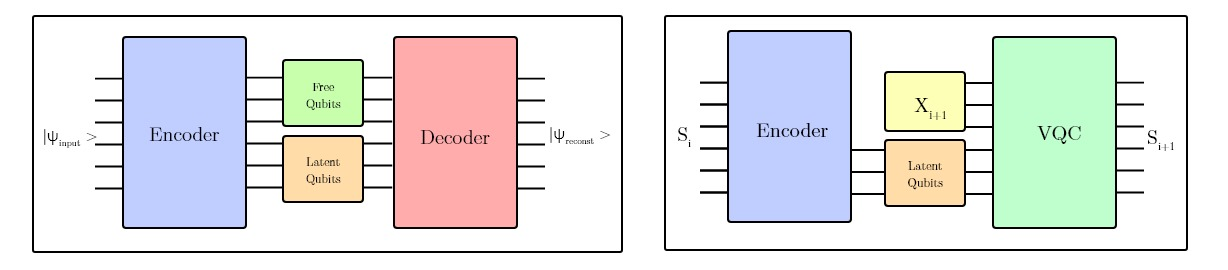
\includegraphics[width=1\linewidth]{model.jpg}
    \caption{Quantum Autoencoder and unit cell of the Model}
    \label{fig:enter-label}
\end{figure*}
The data used in this research was sourced from Yahoo Finance, covering the S\&P 500 indices for major corporations in the United States \cite{b9}. The dataset contains data of 505 stocks It includes daily records from February 2013 to February 2023, detailing key metrics such as the opening price, closing price, highest and lowest prices, and trading volumes for both indices. This comprehensive dataset spans over eleven years, providing a substantial amount of information for analysis. Table I shows a preview for the dataset for a single stock named \textit{AAL}.

The dataset was first partitioned into two subsets based on time frames: the training set comprised data from February 2013 to December 2017 for all 505 stocks of S\&P500, while the test set included data from January 2018 to February 2023 for S\&P 500 index. This temporal split ensured that the model was assessed using a completely unseen dataset. This approach simulates real-world forecasting scenarios and provides a strong test of the model's ability to generalize.  

All numerical features were normalized using a Min-Max Scaler to standardize the data and eliminate feature scale discrepancies using the following formula \cite{b10}:


\begin{center}
    $x_{\text{normalized}} = \frac{x - x_{\text{min}}}{x_{\text{max}} - x_{\text{min}}}$
\end{center}

The missing data was removed. This clean and scaled dataset provided the foundation for extracting meaningful patterns and evaluating the model's ability to reconstruct and predict market behaviors.

\begin{table}[h!]
\centering
\caption{Preview of the dataset for the stock: AAL}
\begin{tabular}{llrrrrr}
\textbf{Date} & \textbf{Open} & \textbf{High} & \textbf{Low} & \textbf{Close} & \textbf{Volume(M)}\\
\midrule
2013-02-08 & 15.07 & 15.12 & 14.63 & 14.75 & 8.407 \\
2013-02-11 & 14.89 & 15.01 & 14.26 & 14.46 & 8.882 \\
2013-02-12 & 14.45 & 14.51 & 14.10 & 14.27 & 8.126 \\
2013-02-13 & 14.30 & 14.94 & 14.25 & 14.66 & 10.259 \\
2013-02-14 & 14.94 & 14.96 & 13.16 & 13.99 & 31.879 \\
\bottomrule
\end{tabular}
\end{table}

\begin{table}[h!]
\centering
\caption{Statistical Summary of S\&P 500 from 2018 - 2023}
\begin{tabular}{lccccc}

\textbf{Statistic} & \textbf{Open}   & \textbf{High}   & \textbf{Low}    & \textbf{Close}  & \textbf{Volume}           \\
\midrule
Count     & 1284    & 1284    & 1284    & 1284    & 1284  \\ 
Mean      & 3460.05 & 3481.54 & 3436.69 & 3460.38 & $4.23 \times 10^9$ \\ 
Std       & 666.46  & 670.13  & 662.89  & 666.81  & $1.07 \times 10^9$ \\ 
Min       & 2290.71 & 2300.73 & 2191.86 & 2237.40 & $1.30 \times 10^9$ \\ 
Max       & 4804.51 & 4818.62 & 4780.04 & 4796.56 & $9.98 \times 10^9$ \\ \hline
\end{tabular}
\end{table}
The open price represents the asset's value at the beginning of the trading session, providing insight into initial market sentiment \cite{b11}. The high is the highest price reached during the trading period, reflecting market peaks, while the low is the lowest price, showing market dips \cite{b12}. The close price is particularly significant, as it indicates the final trading price of the day, often used for trend analysis and forecasting \cite{b13}. Lastly, volume measures the total number of shares or contracts traded, helping to gauge market liquidity and investor interest. When combined, these metrics provide traders and analysts with a comprehensive view of market trends, momentum, and sentiment \cite{b14}.

The S\&P 500 index is calculated using a market capitalization-weighted methodology. Each constituent company’s weight in the index is determined by its market capitalization, which is the product of the company’s stock price and the number of shares outstanding. The formula used for calculating the index value involves summing the market capitalizations of all 505 companies in the index and then dividing that sum by a divisor, which is adjusted for stock splits, mergers, and other corporate actions \cite{b15}. 

This calculation method allows the S\&P 500 to reflect the overall performance of the largest U.S. companies, providing a benchmark for the U.S. stock market as a whole \cite{b16}.

\section{Methodology}
The objective of this study is to forecast the closing price of the S\&P 500 index for any trading day by utilizing historical data from the previous $k$ trading days. Each trading day consists of 5 attributes: open price, close price, low price, high price, and the volume traded.

The model operates on a sequence of $k$ feature vectors, each having a length of 5. These vectors are constructed from data over a sliding window of $k$ consecutive days, providing the model with temporal context and patterns inherent in the market's behavior. Using this sequence as input, the model predicts the closing price for the next trading day, leveraging historical trends and inter-dependencies among the features.

The model comprises a quantum encoder and a series of quantum variational circuits (QVCs), as in Fig 1. The quantum autoencoder is trained on all 5 length feature vectors by minimizing the reconstruction loss \cite{b17}.

The quantum encoder takes an \(n\)-qubit quantum state \(|\psi\rangle \in \mathcal{H}_n\), where \(\mathcal{H}_n\) is the \(2^n\)-dimensional Hilbert space. A unitary transformation \(U\) is applied to map the state into a smaller Hilbert space, \(\mathcal{H}_k \subset \mathcal{H}_n\), of dimension \(2^k\). The latent qubits consisting of k qubits represents the latent space of dimension \(2^k\). The remaining \(n-k\) qubits ideally are supposed to be data-free.
 While the encoder helps reduce interference with state data, its repeated use can introduce potential errors due to the additional gates involved. Now, we inject new data into these \(n-k\) qubits for the next data. The first $n - k$ components of the feature vector are the angle embedded to free qubits in the X-axis and the remaining components in the Y-axis of the free qubits. Each feature vector should be less than twice of the number of free qubits.
\begin{figure}
    \centering
    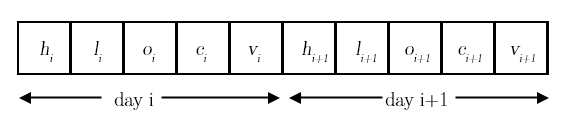
\includegraphics[width=1\linewidth]{feature vector.png}
    \caption{A feature vector by clubbing two day data}
    \label{fig:enter-label}
\end{figure}

The model also clubs multiple time frames to inject as shown in Fig 2. Clubbing multiple days' data into a single input for a machine learning model helps capture broader temporal trends, which is essential for forecasting tasks such as stock market prediction. By aggregating data from consecutive days, the model can focus on longer-term patterns, which are often more predictive than the daily fluctuations seen in financial markets. This approach reduces the impact of noise that may arise from short-term volatility, providing a more stable and reliable feature set for the model to learn from. It makes data more interpretable and reducing overfitting. As a result, clubbing multiple days' data enhances the model's ability to generalize and predict future behavior more effectively \cite{b18}.

The data processed by the $i$-th cell, denoted as $S_i$, is fed into an encoder that compresses it into a smaller number of qubits. The next feature vector, $X_{i+1}$, is then injected into the remaining free qubits. After this, the data undergoes processing by a Quantum Variational Circuit (QVC) and becomes available for the subsequent cell. This process continues in a cell-by-cell manner, where each cell processes its corresponding data and passes it on to the next.

The model is trained on all 505 stocks from February 2013 to December 2017. Firstly, all the feature vectors obtained from the sliding window are used to train the quantum autoencoder. Once the autoencoder is trained to produce latent state from an input state, the VQC is trained to predict the next-day closing price of the stock \cite{b18}. In the autoencoder experiment, 5 qubits were utilized for 1-day clubbing, while 10 qubits were used for both 2-day and 3-day clubbing.

The autoencoder is trained for 300 epochs. After training the auto-encoder, the model is trained for 200 epochs against the closing price prediction. The test group consists of S\&P 500 index from January 2018 to February 2023 covering the COVID-19 pandemic \cite{b19}.

The model was trained using PennyLane's default.qubit, a basic state simulator for qubit-based quantum circuits. Each experiment was conducted on a machine with 10 cores and 20 GB of RAM. The training employed PyTorch's RMSProp optimizer with a learning rate of 0.01, using Mean Squared Error (MSE) as the loss function. Each experiment took around 15 hours with the given configurations.

 \section{Results}
 The R² score, or coefficient of determination, was chosen as the primary performance indicator to evaluate the model's fit and predictive accuracy. This metric quantifies the proportion of variance in the dependent variable that the model explains, making it particularly suitable for time series data where capturing trends and seasonality is crucial \cite{b20}. An R² score close to 1 indicates that the model successfully accounts for the variability in the data, while a score near 0 suggests limited explanatory power. It is given by the following formula:
\[R^2 = 1 - \frac{\sum_{i=1}^n (y_i - \hat{y}_i)^2}{\sum_{i=1}^n (y_i - \bar{y})^2}\]
\begin{figure*}[ht]
    \centering
    \begin{subfigure}[b]{0.48\textwidth}
        \centering
        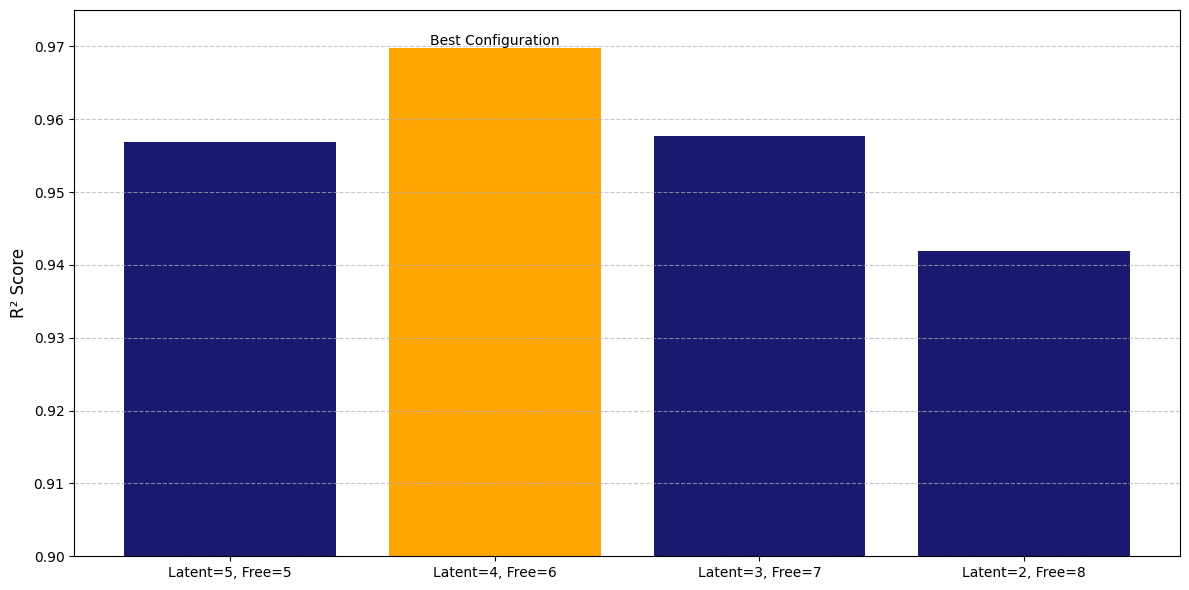
\includegraphics[width=\textwidth]{configs.png}
        \caption{R² Scores for Different Latent and Free Qubit Configurations}
    \end{subfigure}
    %
    \begin{subfigure}[b]{0.48\textwidth}
        \centering
        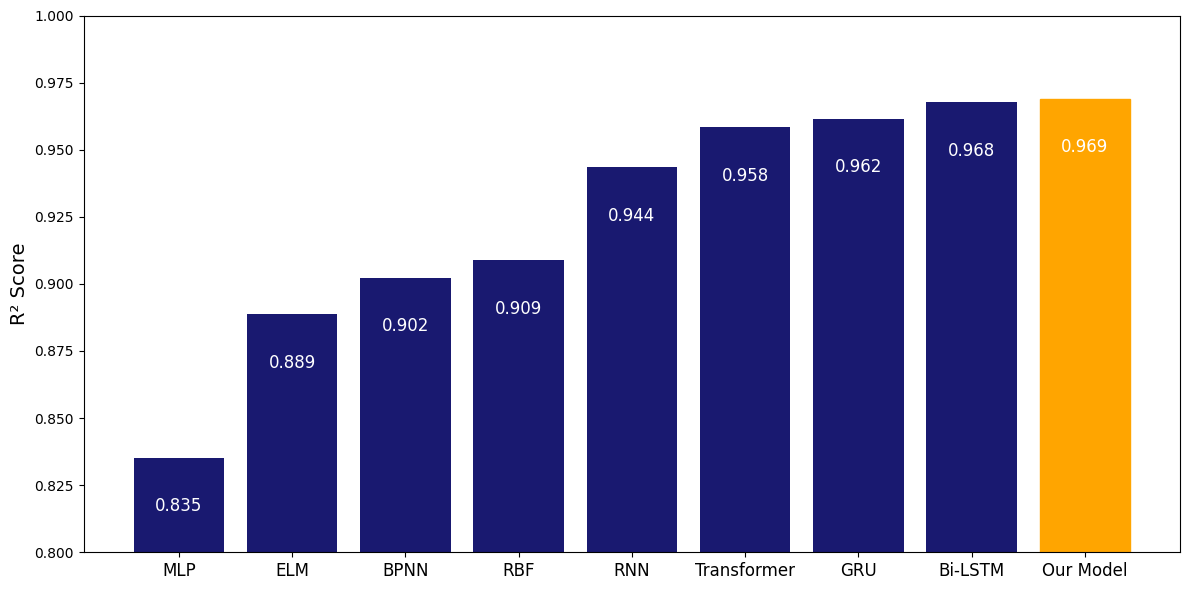
\includegraphics[width=\textwidth]{compar.png}
        \caption{Comparison of Test Set R² Scores Across Models}
    \end{subfigure}
\end{figure*}

\begin{figure*}
    \centering
    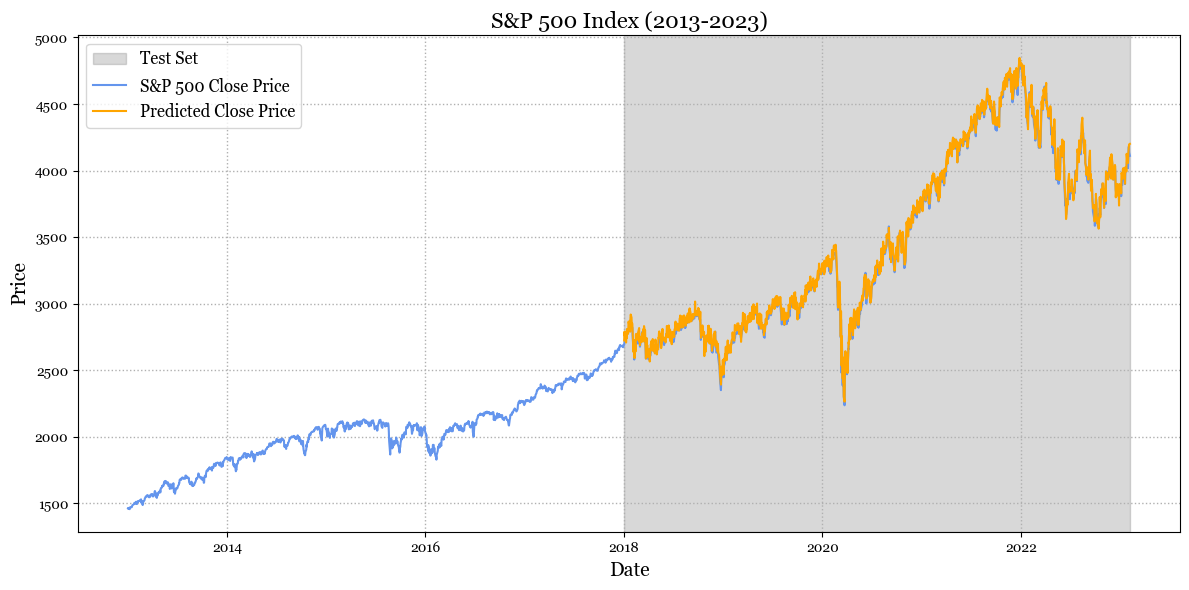
\includegraphics[width=1\linewidth]{plot.png}
    \caption{S\&P 500 close price from 2013 to 2023}
    \label{fig:enter-label}
\end{figure*}

We trained our model using various configurations of the autoencoder by adjusting the latent-free qubit ratio. For this experiment, we aggregated the data into two-day intervals and evaluated the model under different settings. The results of these configurations are presented in Figure 3, highlighting the impact of varying the latent-free qubit ratio on the model's performance.

\begin{table}[ht]
    \centering
    \caption{R\textsuperscript{2} scores for different levels of data clubbing}
    \begin{tabular}{|c|c|}
        \hline
        \textbf{Days Clubbed} & \textbf{R\textsuperscript{2} Score} \\ \hline
        1 Day                & 0.967                               \\ \hline
        2 Days               & 0.969                               \\ \hline
        3 Days               & 0.272                               \\ \hline
    \end{tabular}
    
\end{table}


We further trained our model using varying levels of data aggregation to analyze the impact of clubbing multiple days of data on performance. Table 2 summarizes the R² scores for 1-day, 2-day, and 3-day clubbing configurations. The results demonstrate that 1-day and 2-day clubbing yielded high R² scores of 0.967 and 0.969, respectively, indicating strong predictive performance. However, the R² score dropped significantly to 0.272 for 3-day clubbing, suggesting a loss of predictive capability with increased aggregation.

\begin{table}[ht]
    \centering
    \begin{tabular}{l c}
        \toprule
        \textbf{Model} & \textbf{R² Score} \\
        \midrule
        MLP            & 0.8353            \\
        ELM            & 0.8888            \\
        BPNN           & 0.9023            \\
        RBF            & 0.9089            \\
        RNN            & 0.9436            \\
        Transformer    & 0.9584            \\
        GRU            & 0.9616            \\
        Bi-LSTM        & 0.9678            \\
        \textbf{Our Model} & \textbf{0.9690} \\
        \bottomrule
    \end{tabular}
    \caption{Test Set R² Scores for Different Models}
    \label{tab:r2_scores}
\end{table}

The comparison of R² scores on the test set for various models reveals that our model outperforms all others, achieving an R² score of 0.969. Among the other models, Bi-LSTM demonstrates the second-best performance with an R² of 0.9678, followed closely by GRU at 0.9616 and Transformer at 0.9584. Traditional models such as MLP, ELM, and RBF exhibit lower R² scores, indicating that they struggle to capture the complex patterns in the data, with scores of 0.8353, 0.8888, and 0.9089, respectively. Deep learning models like RNN also perform well, with an R² of 0.9436, but they still fall short of our model's performance \cite{b21}. These results highlight the superiority of our model in handling the challenges of financial time series forecasting, with its ability to capture long-term dependencies and intricate patterns in the data, leading to the highest R² score among all tested models.

\section{Conclusion}
In this work, we present a quantum autoencoder-based model for the task of predicting the S\&P 500 index. We demonstrate the performance of our model on financial time series data, showcasing its ability to capture intricate patterns and temporal dependencies. Our results highlight the superior predictive accuracy of our model compared to traditional machine learning techniques, achieving a high R² score of 0.969 on the test set. This work paves the way for further advancements in applying quantum machine learning techniques to financial forecasting, offering a promising solution for predicting stock market trends with high accuracy.
\begin{thebibliography}{00}
\bibitem{b1} Ali, Muhammad, et al. "Prediction of complex stock market data using an improved hybrid emd-lstm model." Applied Sciences 13.3 (2023): 1429.
\bibitem{b2} Ahangar, Reza Gharoie, Mahmood Yahyazadehfar, and Hassan Pournaghshband. "The comparison of methods artificial neural network with linear regression using specific variables for prediction stock price in Tehran stock exchange." arXiv preprint arXiv:1003.1457 (2010).
\bibitem{b3} Mintarya, Latrisha N., et al. "Machine learning approaches in stock market prediction: A systematic literature review." Procedia Computer Science 216 (2023): 96-102.
\bibitem{b4} Nti, Isaac Kofi, Adebayo Felix Adekoya, and Benjamin Asubam Weyori. "A systematic review of fundamental and technical analysis of stock market predictions." Artificial Intelligence Review 53.4 (2020): 3007-3057.
\bibitem{b5} Farhi, Edward, Jeffrey Goldstone, and Sam Gutmann. "A quantum approximate optimization algorithm." arXiv preprint arXiv:1411.4028 (2014).
\bibitem{b6} Biamonte, Jacob, et al. "Quantum machine learning." Nature 549.7671 (2017): 195-202.
\bibitem{b7} Mitarai, Kosuke, et al. "Quantum circuit learning." Physical Review A 98.3 (2018): 032309.
\bibitem{b8} Nielsen, Michael A., and Isaac L. Chuang. Quantum computation and quantum information. Cambridge university press, 2010.
\bibitem{b9} Finance, Yahoo. "Yahoo Finance." Retrieved from finance. yahoo. com: https://finance. yahoo. com/recent-quotes (2020).
\bibitem{b10} Pedregosa, Fabian, et al. "Scikit-learn: Machine learning in Python." the Journal of machine Learning research 12 (2011): 2825-2830.
\bibitem{b11} Bodie, Zvi, Alex Kane, and Alan Marcus. Ebook: Investments-global edition. McGraw Hill, 2014.
\bibitem{b12} Hull, John C. "Options, futures, and other derivatives (Ninth)." (2015).
\bibitem{b13} Pring, Martin J. Study guide for technical analysis explained. Vol. 5. New York: McGraw-Hill, 2002.
\bibitem{b14} Malkiel, Burton Gordon. The random walk guide to investing: Ten rules for financial success. WW Norton \& Company, 2003.
\bibitem{b15} Serhiienko, Olena, Tetyana Novikova, and Vyacheslav Lyashenko. "Comparative Analysis of the Dynamics of Futures for the Dow Jones, S\&P 500 and Nasdaq." (2023).
\bibitem{b16} Rahman, Matiur. "Interactions between Equity REITs and S\&P 500 Returns." International Journal of Economics and Financial Issues 14.3 (2024): 206-211.
\bibitem{b17} Silver, Daniel, et al. "LEXIQL: Quantum Natural Language Processing on NISQ-era Machines." 2024 SC24: International Conference for High Performance Computing, Networking, Storage and Analysis SC. IEEE Computer Society, 2024.
\bibitem{b18} Shen, Zhipeng, et al. "A novel time series forecasting model with deep learning." Neurocomputing 396 (2020): 302-313.
\bibitem{b19} Fernandez-Perez, Adrian, et al. "COVID-19 pandemic and stock market response: A culture effect." Journal of behavioral and experimental finance 29 (2021): 100454.
\bibitem{b20} Hyndman, R. J. Forecasting: principles and practice. OTexts, 2018.
\bibitem{b21} Ge, Qing. "Enhancing stock market Forecasting: A hybrid model for accurate prediction of S\&P 500 and CSI 300 future prices." Expert Systems with Applications 260 (2025): 125380.

\end{thebibliography}
\vspace{12pt}

\end{document}
